\documentclass[11pt]{beamer}
\title{SBFSEM-tools tutorial}
\author{Sara Patterson}
\institute{Neitz Lab, University of Washington}
\usetheme{Goettingen}

\usepackage[utf8]{inputenc}
\usepackage[T1]{fontenc}
\usepackage[english]{babel}
\usepackage{amsmath}
\usepackage{amsfonts}
\usepackage{amssymb}
\usepackage{siunitx}
\usepackage{graphicx}
\usepackage{listings}
\usepackage{hyperref}

\definecolor{codegreen}{rgb}{0,0.6,0}
\definecolor{codegray}{rgb}{0.5,0.5,0.5}
\definecolor{codepurple}{rgb}{0.58,0,0.82}
\definecolor{backcolour}{rgb}{0.95,0.95,0.92}

\lstdefinestyle{mystyle}{
	backgroundcolor=\color{backcolour},   
	commentstyle=\color{codegreen},
	keywordstyle=\color{magenta},
	numberstyle=\tiny\color{codegray},
	stringstyle=\color{codepurple},
	basicstyle=\footnotesize,
	breakatwhitespace=false,         
	breaklines=true,                 
	captionpos=b,                    
	keepspaces=true,                 
	numbers=left,                    
	numbersep=5pt,                  
	showspaces=false,                
	showstringspaces=false,
	showtabs=false,                  
	tabsize=2
}
\lstset{style=mystyle}

\begin{document}
% --------------------------------------------------- Slide --
	\maketitle
% --------------------------------------------------- Slide --
%	\tableofcontents
% --------------------------------------------------- Slide --
% ------------------------------------------------- Section --
\section{SBFSEM-tools}
% ------------------------------------------------- Section --
\begin{frame}
	\frametitle{SBFSEM-tools}
	Goal: basic analysis support requiring minimal setup and background in computers, math, etc.
	\vskip10pt
	Current capabilities:
	\begin{itemize}
		\item Import and parse data into Matlab through Viking's OData service
		\item Parse data into high-level data structures (Neuron, etc)
		\item Count up synapses and condense synapses spanning multiple slices 
		\item Summarize synapses with statistics and plots
		\item Arbitrary geometry rendering
		\item Basic network analysis
	\end{itemize}
\end{frame}
% --------------------------------------------------- Slide --
% ------------------------------------------------- Section -- 
\section{Install}
% ------------------------------------------------- Section -- 
% --------------------------------------------------- Slide --
\begin{frame}[fragile]
	\frametitle{Install}
	First download or clone \href{www.github.com/sarastokes/sbfsem-tools}{\textcolor{blue}{SBFSEM-tools}}.
	
	Make sure SBSFEM-tools is added to your MATLAB \href{https://www.mathworks.com/help/matlab/ref/addpath.html}{\textcolor{blue}{path}} like so:
	\begin{lstlisting}[language=matlab]	
	addpath(genpath('C:\...\sbfsem-tools'));\end{lstlisting}
	If you already have JSONLab installed, make sure 
	\begin{lstlisting}[language=matlab] 
	which loadjson\end{lstlisting} 
	returns the version in sbfsem-tools. Otherwise, you might get some errors.
\end{frame}
% --------------------------------------------------- Slide --
% ------------------------------------------------- Section -- 
\section{Neuron Class}
% ------------------------------------------------- Section -- 
% --------------------------------------------------- Slide --
\begin{frame}[fragile]
	\frametitle{Neuron}
	The Neuron class is the basic representation of a cell exported from Viking. To create a Neuron:
\begin{lstlisting}[language=matlab]
% cellName = Neuron(cellID, 'source');
c207 = Neuron(207, 'temporal');\end{lstlisting}
Note: Source can be `inferior', `temporal' or `rc1'. Also, abbreviating to `i', `t' and `r' works as well.\\
Open the Neuron class in the user interface
\begin{lstlisting}[language=matlab]
NeuronApp(c207);\end{lstlisting}
To update a neuron in the workspace:
\begin{lstlisting}[language=matlab]
c207.update();\end{lstlisting}
\end{frame}
% --------------------------------------------------- Slide --
\begin{frame}[fragile]
	\frametitle{Neuron}
	\framesubtitle{Properties}
	Neuron has the following publicly accessible properties:
	\begin{itemize}
		\item data
		\item \texttt{viking} - Structure of the neuron's info from viking
		\item \texttt{nodes} - Table of all annotations
		\item \texttt{edges} - Table of links between annotations
		\item \texttt{volumeScale} - Units are nm/pix for X,Y and nm/section for Z
		\item \texttt{synapses} - Table of each child structure.
		\item \texttt{geometries} - Table of closed curve geometries
		\item \texttt{analysis} - Containers.map of analyses
		\item \texttt{lastModified} - Last update of neuron from OData
	\end{itemize}
\end{frame}
% --------------------------------------------------- Slide --
\begin{frame}[fragile]
	\frametitle{NeuronGroup}
	Create a single data object to hold related Neurons. Note inputs can be ID numbers or existing Neurons.
	\begin{lstlisting}[language=matlab]
	h1hc = sbfsem.NeuronGroup([28, 447, 619]);
	% Add a neuron to an existing group
	h1hc.add(4568);
	% Remove a neuron
	h1hc.remove(4568);\end{lstlisting}
\end{frame}
% --------------------------------------------------- Slide --
\begin{frame}[fragile]
	\frametitle{NeuronGroup}
	\framesubtitle{Methods}
	To plot the somas of all Neurons in the NeuronGroup:
	\begin{lstlisting}[language=matlab]
	h1hc.somaPlot();
	h1hc.somaPlot('addLabel',true); % Label with ID
	h1hc.somaPlot('ax',gca); % Add to existing axis
	% Two methods for controlling plot color:
	h1hc.somaPlot('Color', [0 0.8 0.3]);
	h1hc.setPlotColor([0 0.8 0.3]); h1hc.somaPlot;\end{lstlisting}
	\begin{columns}
		\column[]{0.3\textwidth}
			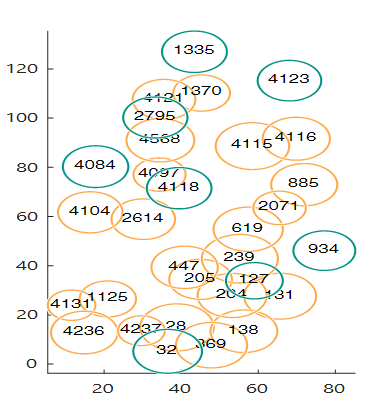
\includegraphics[height=0.4\textheight]{h1h2mosaic}
		\column[]{0.7\textwidth}
			Mosaic of H1 and H2 somas
	\end{columns}
\end{frame}
% --------------------------------------------------- Slide --
% ------------------------------------------------- Section -- 
\section{Analysis}
% ------------------------------------------------- Section -- 
\begin{frame}
	\frametitle{NeuronAnalysis Class}
	The NeuronAnalysis class helps keep population data organized by managing input parameters and results of common analyses. To create a new analysis, subclass NeuronAnalysis and edit the \texttt{doAnalysis} and \texttt{visualize} methods.
	\vskip10pt
	See \texttt{Tutorial.m} for information on these existing classes:
	\begin{itemize}
		\item \textbf{DendriticFieldHull} - uses convex hull to estimate dendritic field area, includes methods for removing axons prior to analysis.
		\item \textbf{PrimaryDendriteDiameter} - returns the median dendrite diameter at a given distance from the soma.
	\end{itemize}
\end{frame}
% --------------------------------------------------- Slide --
\begin{frame}[fragile]
	\frametitle{Views}
	\begin{lstlisting}[language = matlab]
	c6800 = sbfsem.Neuron(6800, `i');
	sbfsem.ui.StratificationView(c6800);
	c207 = sbfsem.Neuron(207, `i');
	sbfsem.ui.SomaDistanceView(c207);
	c4781 = sbfsem.Neuron(4781, `i');
	sbfsem.ui.NodeView(c4781);
	sbfsem.ui.NodeView(c6800);\end{lstlisting}
\end{frame}
% --------------------------------------------------- Slide --
\begin{frame}[fragile]
	\frametitle{Convert to Graph}
	The dendritic structure can be converted to MATLAB's `graph' and `digraph' classes:
	\begin{lstlisting}[language=matlab]
	c127 = sbfsem.Neuron(127, `i');
	G = graph(c127);
	plot(G, `Layout', `force');
	% Default is undirected, add true for digraph
	G = graph(c127, true);\end{lstlisting}
	See MATLAB's documentation for more information on how to use the %\href{https://www.mathworks.com/help/matlab/graph-and-network-algorithms.html}{\textcolor{blue}{graph class}}.
\end{frame}
% --------------------------------------------------- Slide --
\begin{frame}[fragile]
	\frametitle{IPL Boundary Surfaces}
	\begin{lstlisting}[language=matlab]
inl = sbfsem.core.INLBoundary('i');
% Update marker locations from OData
inl.refresh();
% Create the surface
inl.doAnalysis();
% Plot the surface
plot(inl);\end{lstlisting}
	\begin{center}
		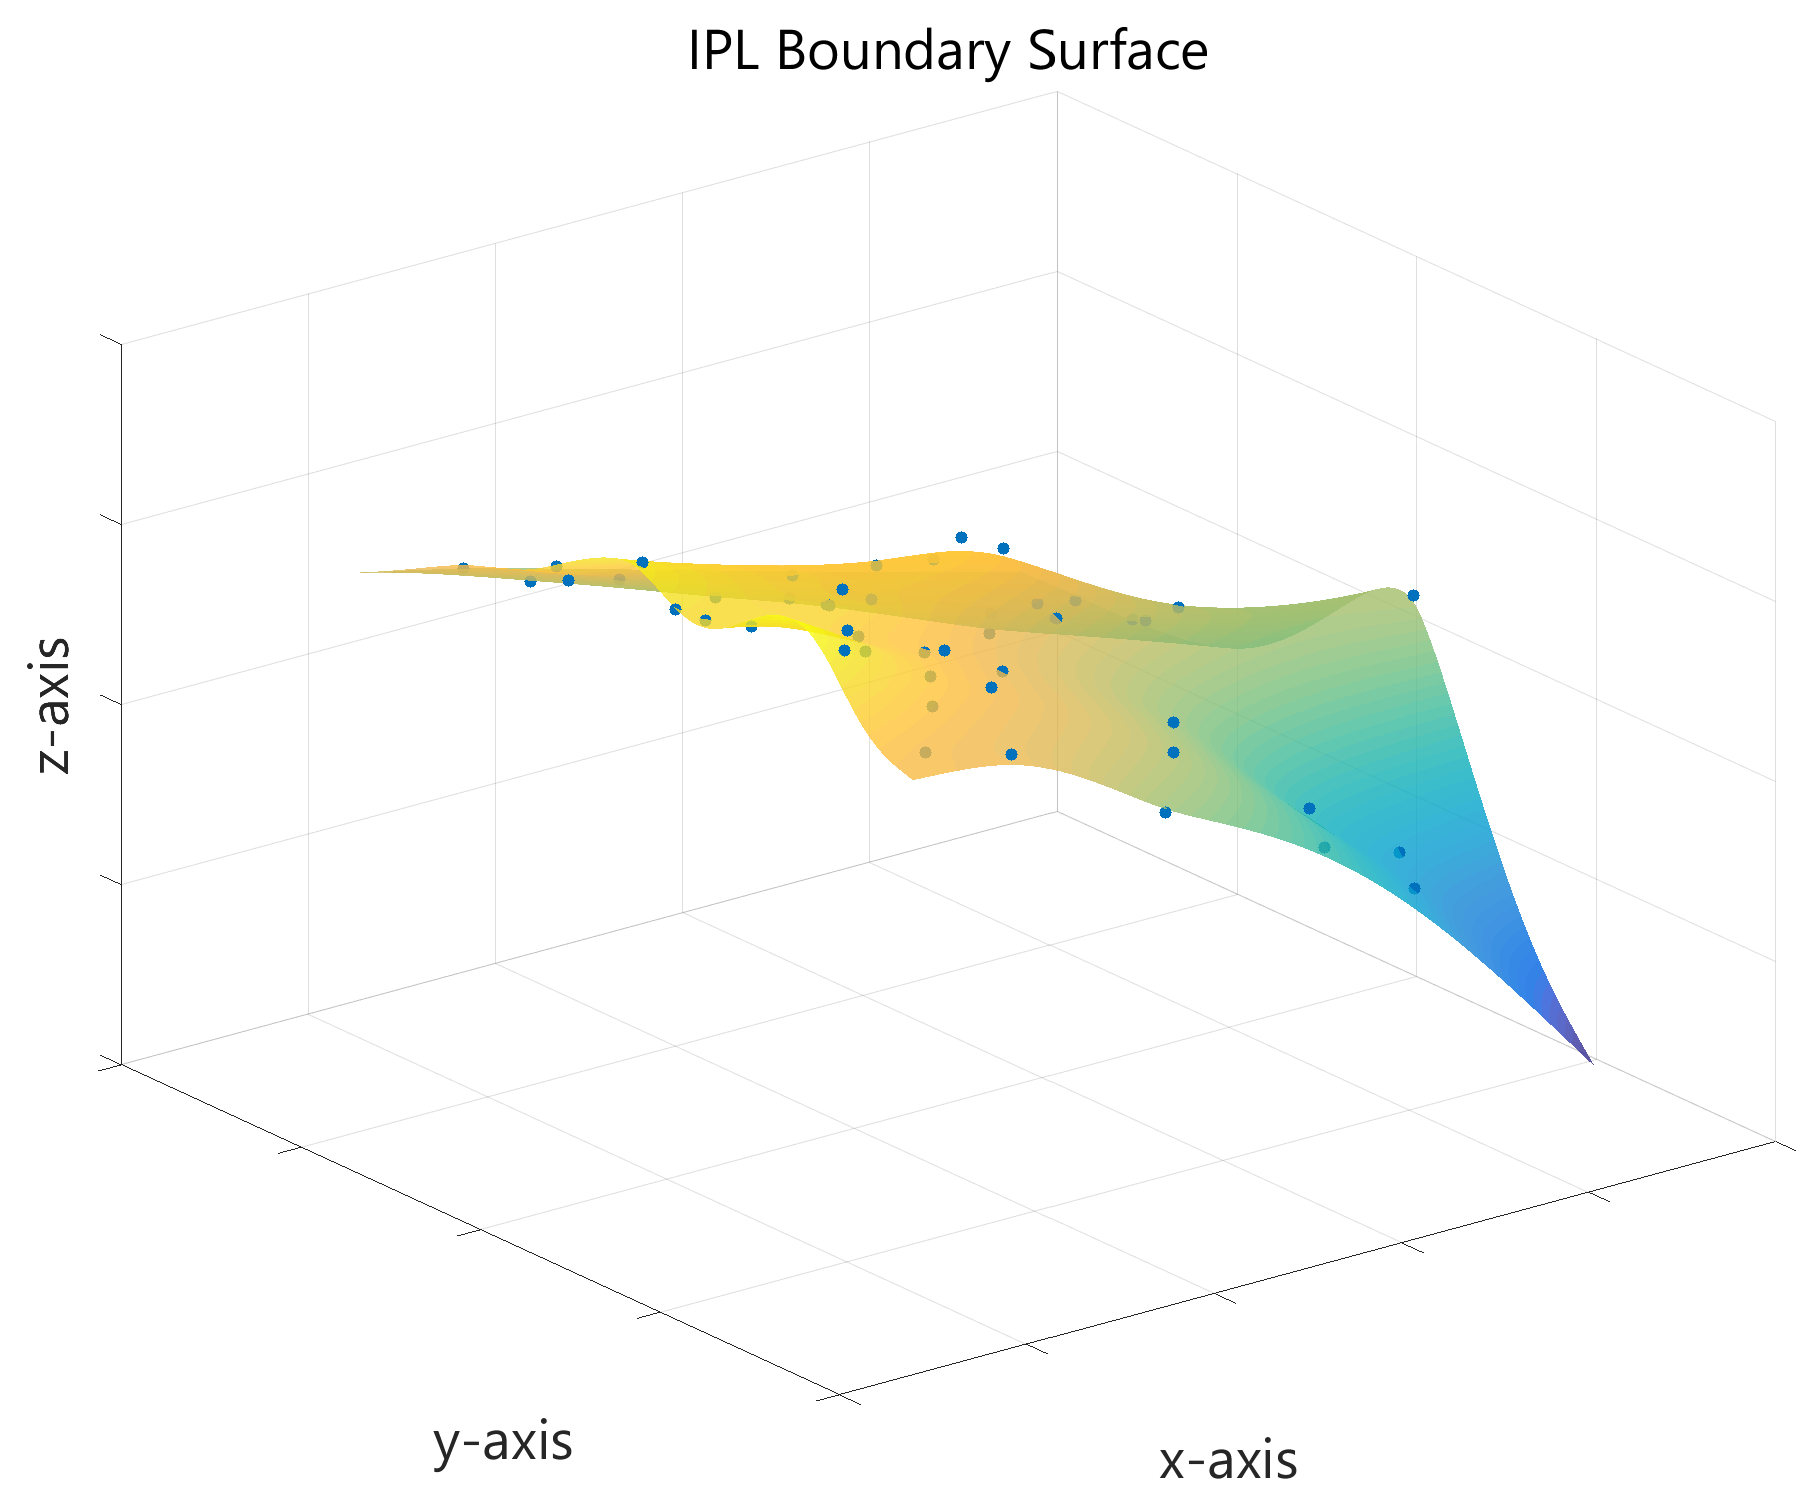
\includegraphics[height=0.4\textheight]{iplboundary}
	\end{center}
\end{frame}
% --------------------------------------------------- Slide --
\begin{frame}[fragile]
	\frametitle{XY Offset}
	The function \textbf{xyRegistration.m} calculates the XY offset through a range of Z sections and outputs statistics on the offsets relative to the most sclerad section input.
	\begin{lstlisting}[language=matlab]
% S xyRegistration(source, [minZ maxZ], plotFlag);
S = xyRegistration('i', [1284 1309], true);\end{lstlisting}
	\begin{columns}
		\column[]{0.55\textwidth}
			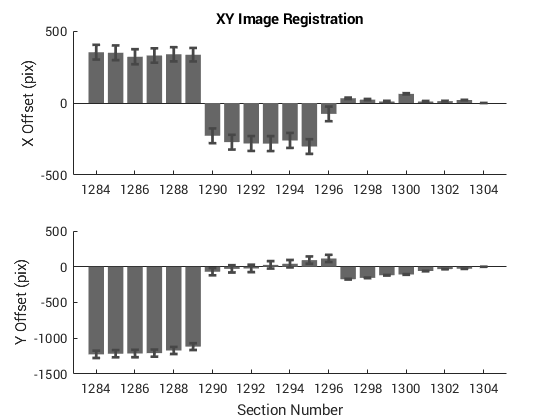
\includegraphics[height=0.4\textheight]{xyAlign}
		\column[]{0.45\textwidth}
			Next on the todo list is a systematic way of applying transforms
	\end{columns}
\end{frame}
% --------------------------------------------------- Slide --
% ------------------------------------------------- Section -- 
\section{Renders}
% ------------------------------------------------- Section -- 
% --------------------------------------------------- Slide --
\begin{frame}
	\frametitle{Renders}
	VikingPlot generates 3D models by fitting the data to three stereotyped geometries - sphere, cylinder and cone. I'm focusing my efforts on the opposite approach - rendering the structures `as is'. By not fitting the data, the renders will be far more accurate. The tradeoff is that this accuracy applies both to the neuron's morphology and the small discrepancies in image registration.
\end{frame}
% --------------------------------------------------- Slide --
\begin{frame}[fragile]
	\frametitle{Closed Curve Renders}
	Closed-curve structures can be rendered into volumes:
	\begin{lstlisting}[language=matlab]
	c2542 = sbfsem.Neuron(2542, `i');
	lmcone = sbfsem.render.ClosedCurve(c2542);\end{lstlisting}
	\begin{center}
		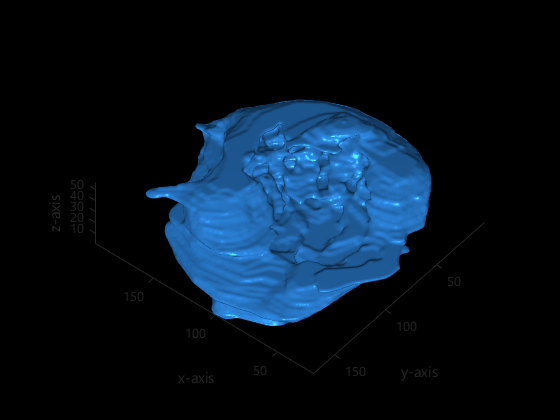
\includegraphics[width=0.4\textwidth]{scone_render}
		\hskip5pt
		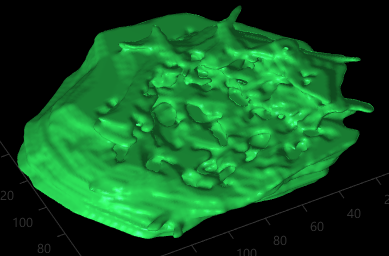
\includegraphics[width=0.4\textwidth]{lmcone_render}
	\end{center}
	See the \texttt{Tutorial.m} file for more information on render colors, lighting and materials.
\end{frame}
% --------------------------------------------------- Slide --
\begin{frame}[fragile]
	\frametitle{Disc Renders}
	\framesubtitle{Rotated Cylinders Method}
	There are two options for disc renders so far.
	\begin{lstlisting}[language=matlab]
	sbfsem.render.Cylinder([c1403, c2578]);\end{lstlisting}
	\begin{columns}
		\column[]{0.55\textwidth}
			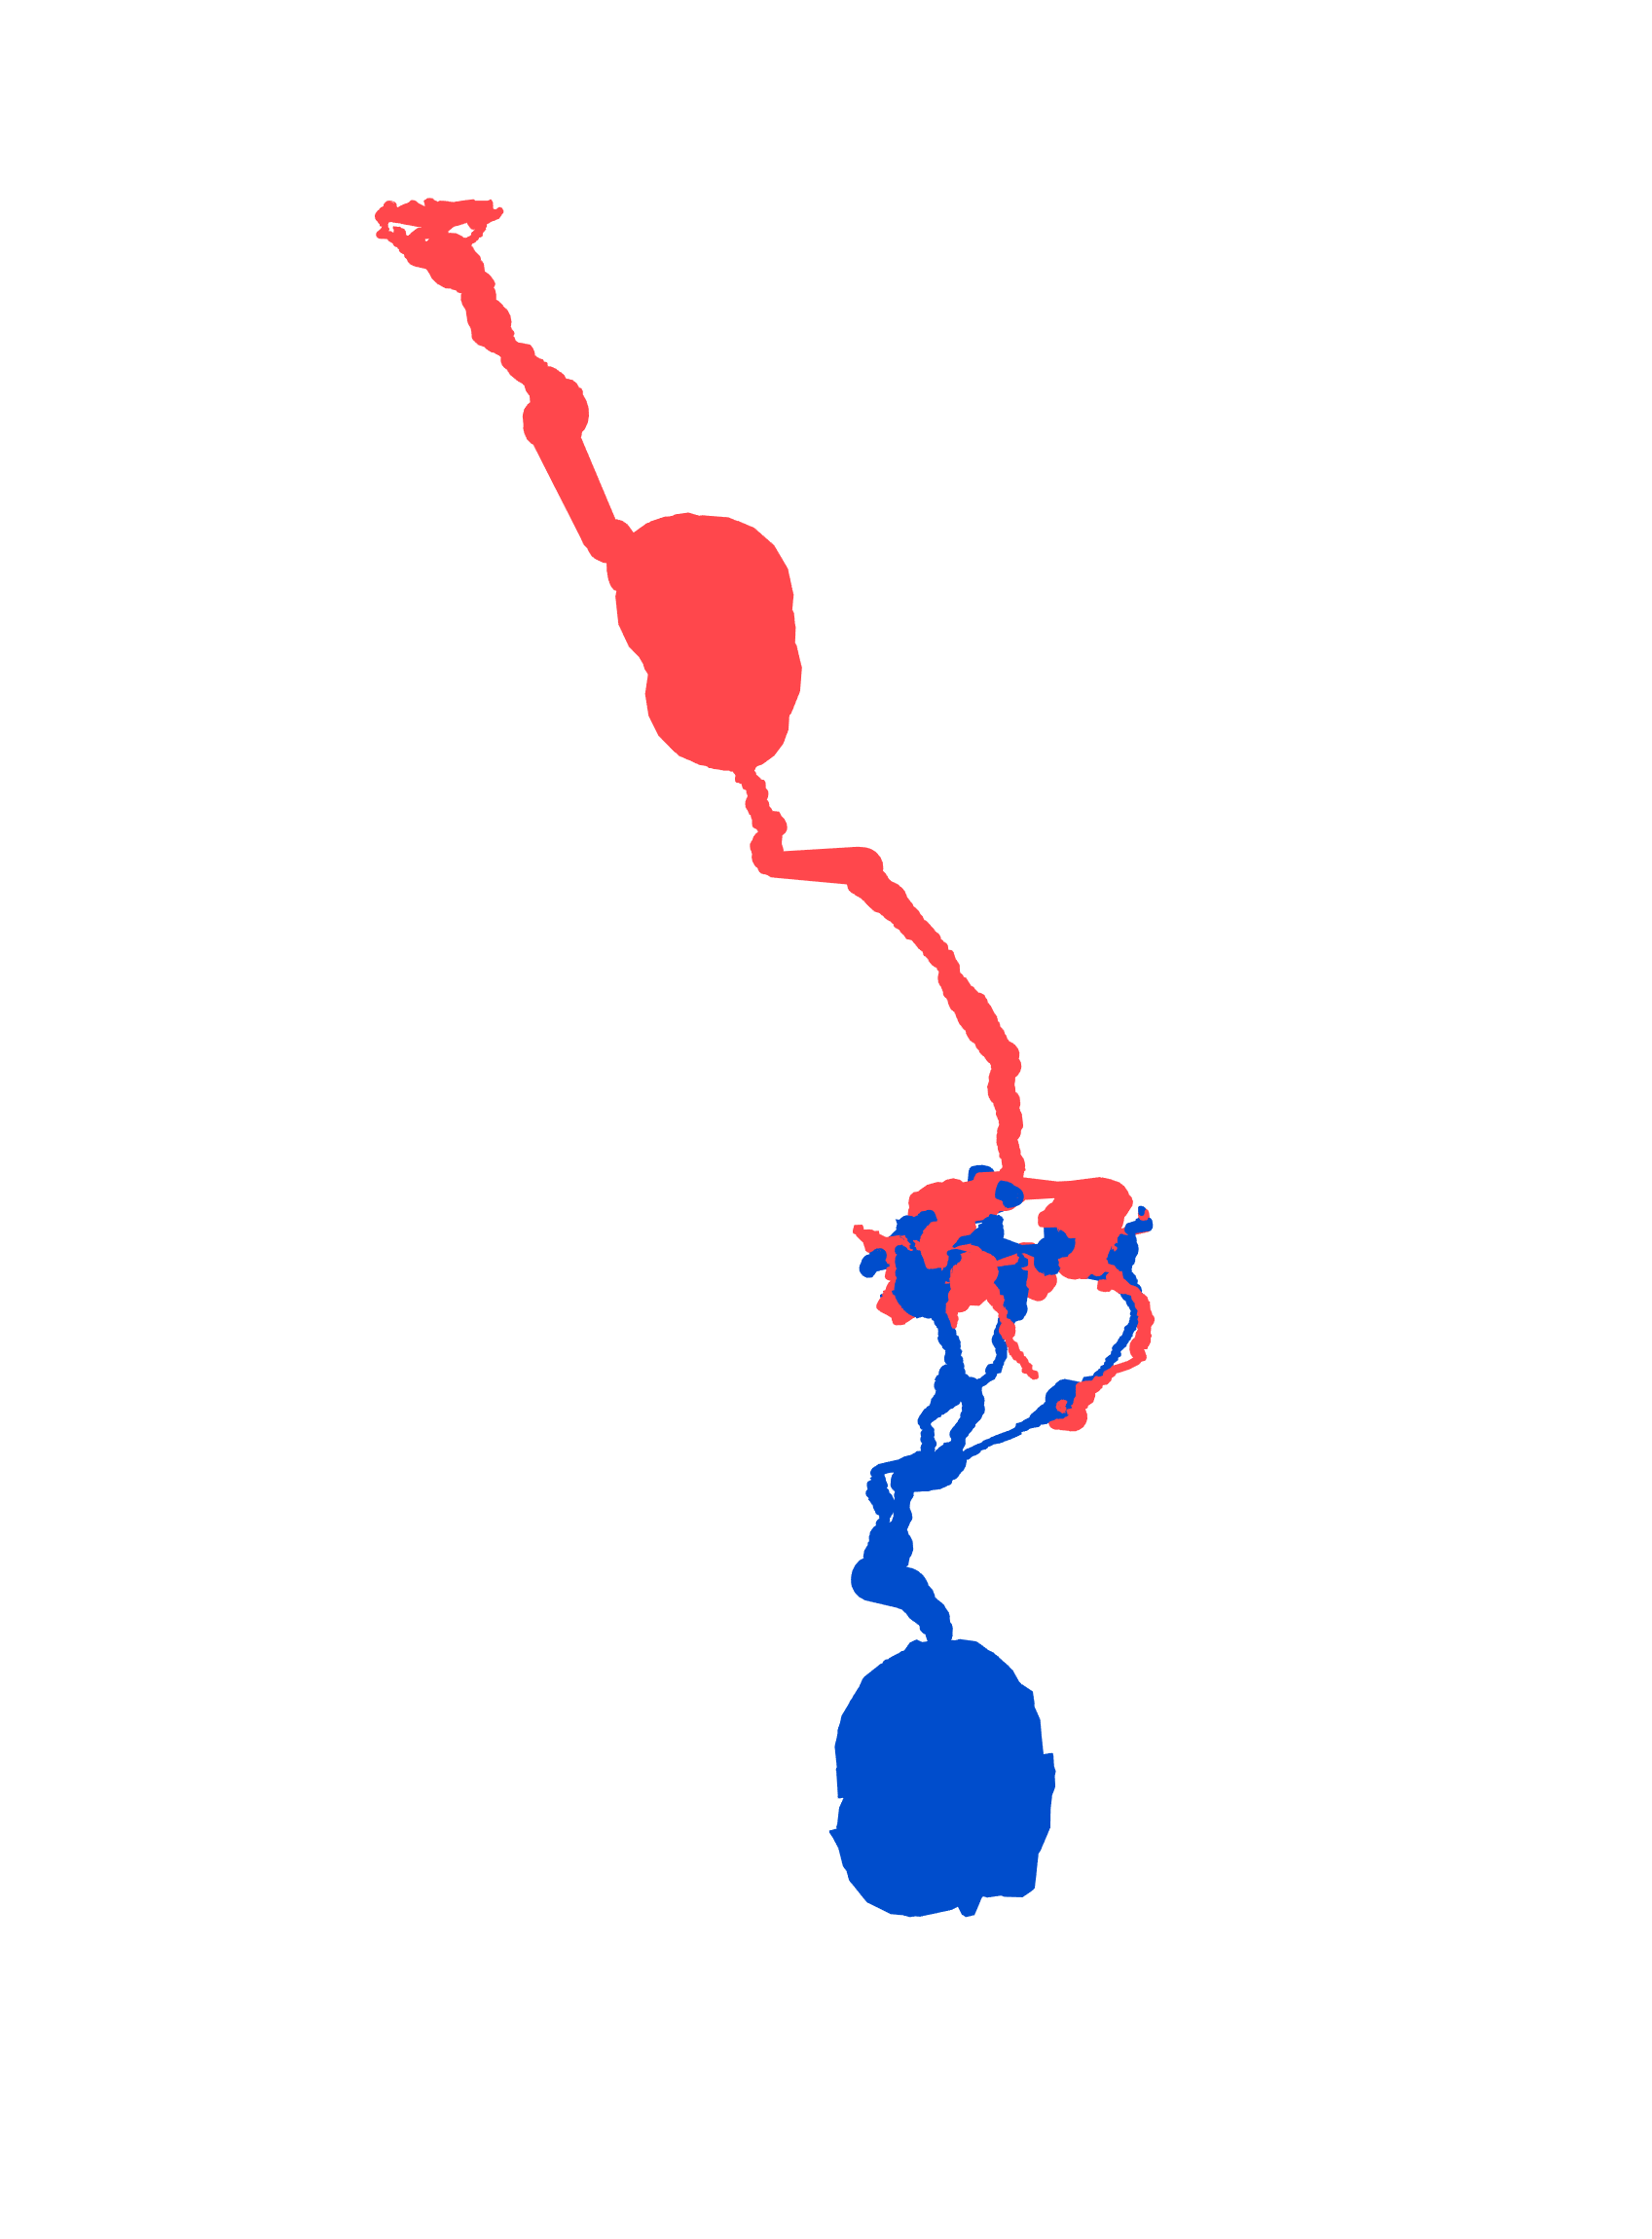
\includegraphics[height=0.45\textheight]{smidget_path}
		\column[]{0.45\textwidth}
			To do:
			\begin{itemize}
				\item Dendrites for Cylinder
				\item Smoothing for Disc
				\item Image registration
			\end{itemize}
	\end{columns}
\end{frame}
% --------------------------------------------------- Slide --
\begin{frame}
	\frametitle{Rotated Cylinders}
	\framesubtitle{Future Work}
	\begin{columns}
		\column[]{0.5\textwidth}
			I'm working on two approaches:
			\begin{itemize}
				\item Optimizing the existing algorithm to reduce the number of odd rotations.
				\item Converting the output to a binary mask volume and remodeling the surface.
			\end{itemize}
		\column[]{0.5\textwidth}
			\includegraphics[width=0.5\textwidth]{midgets2D}
			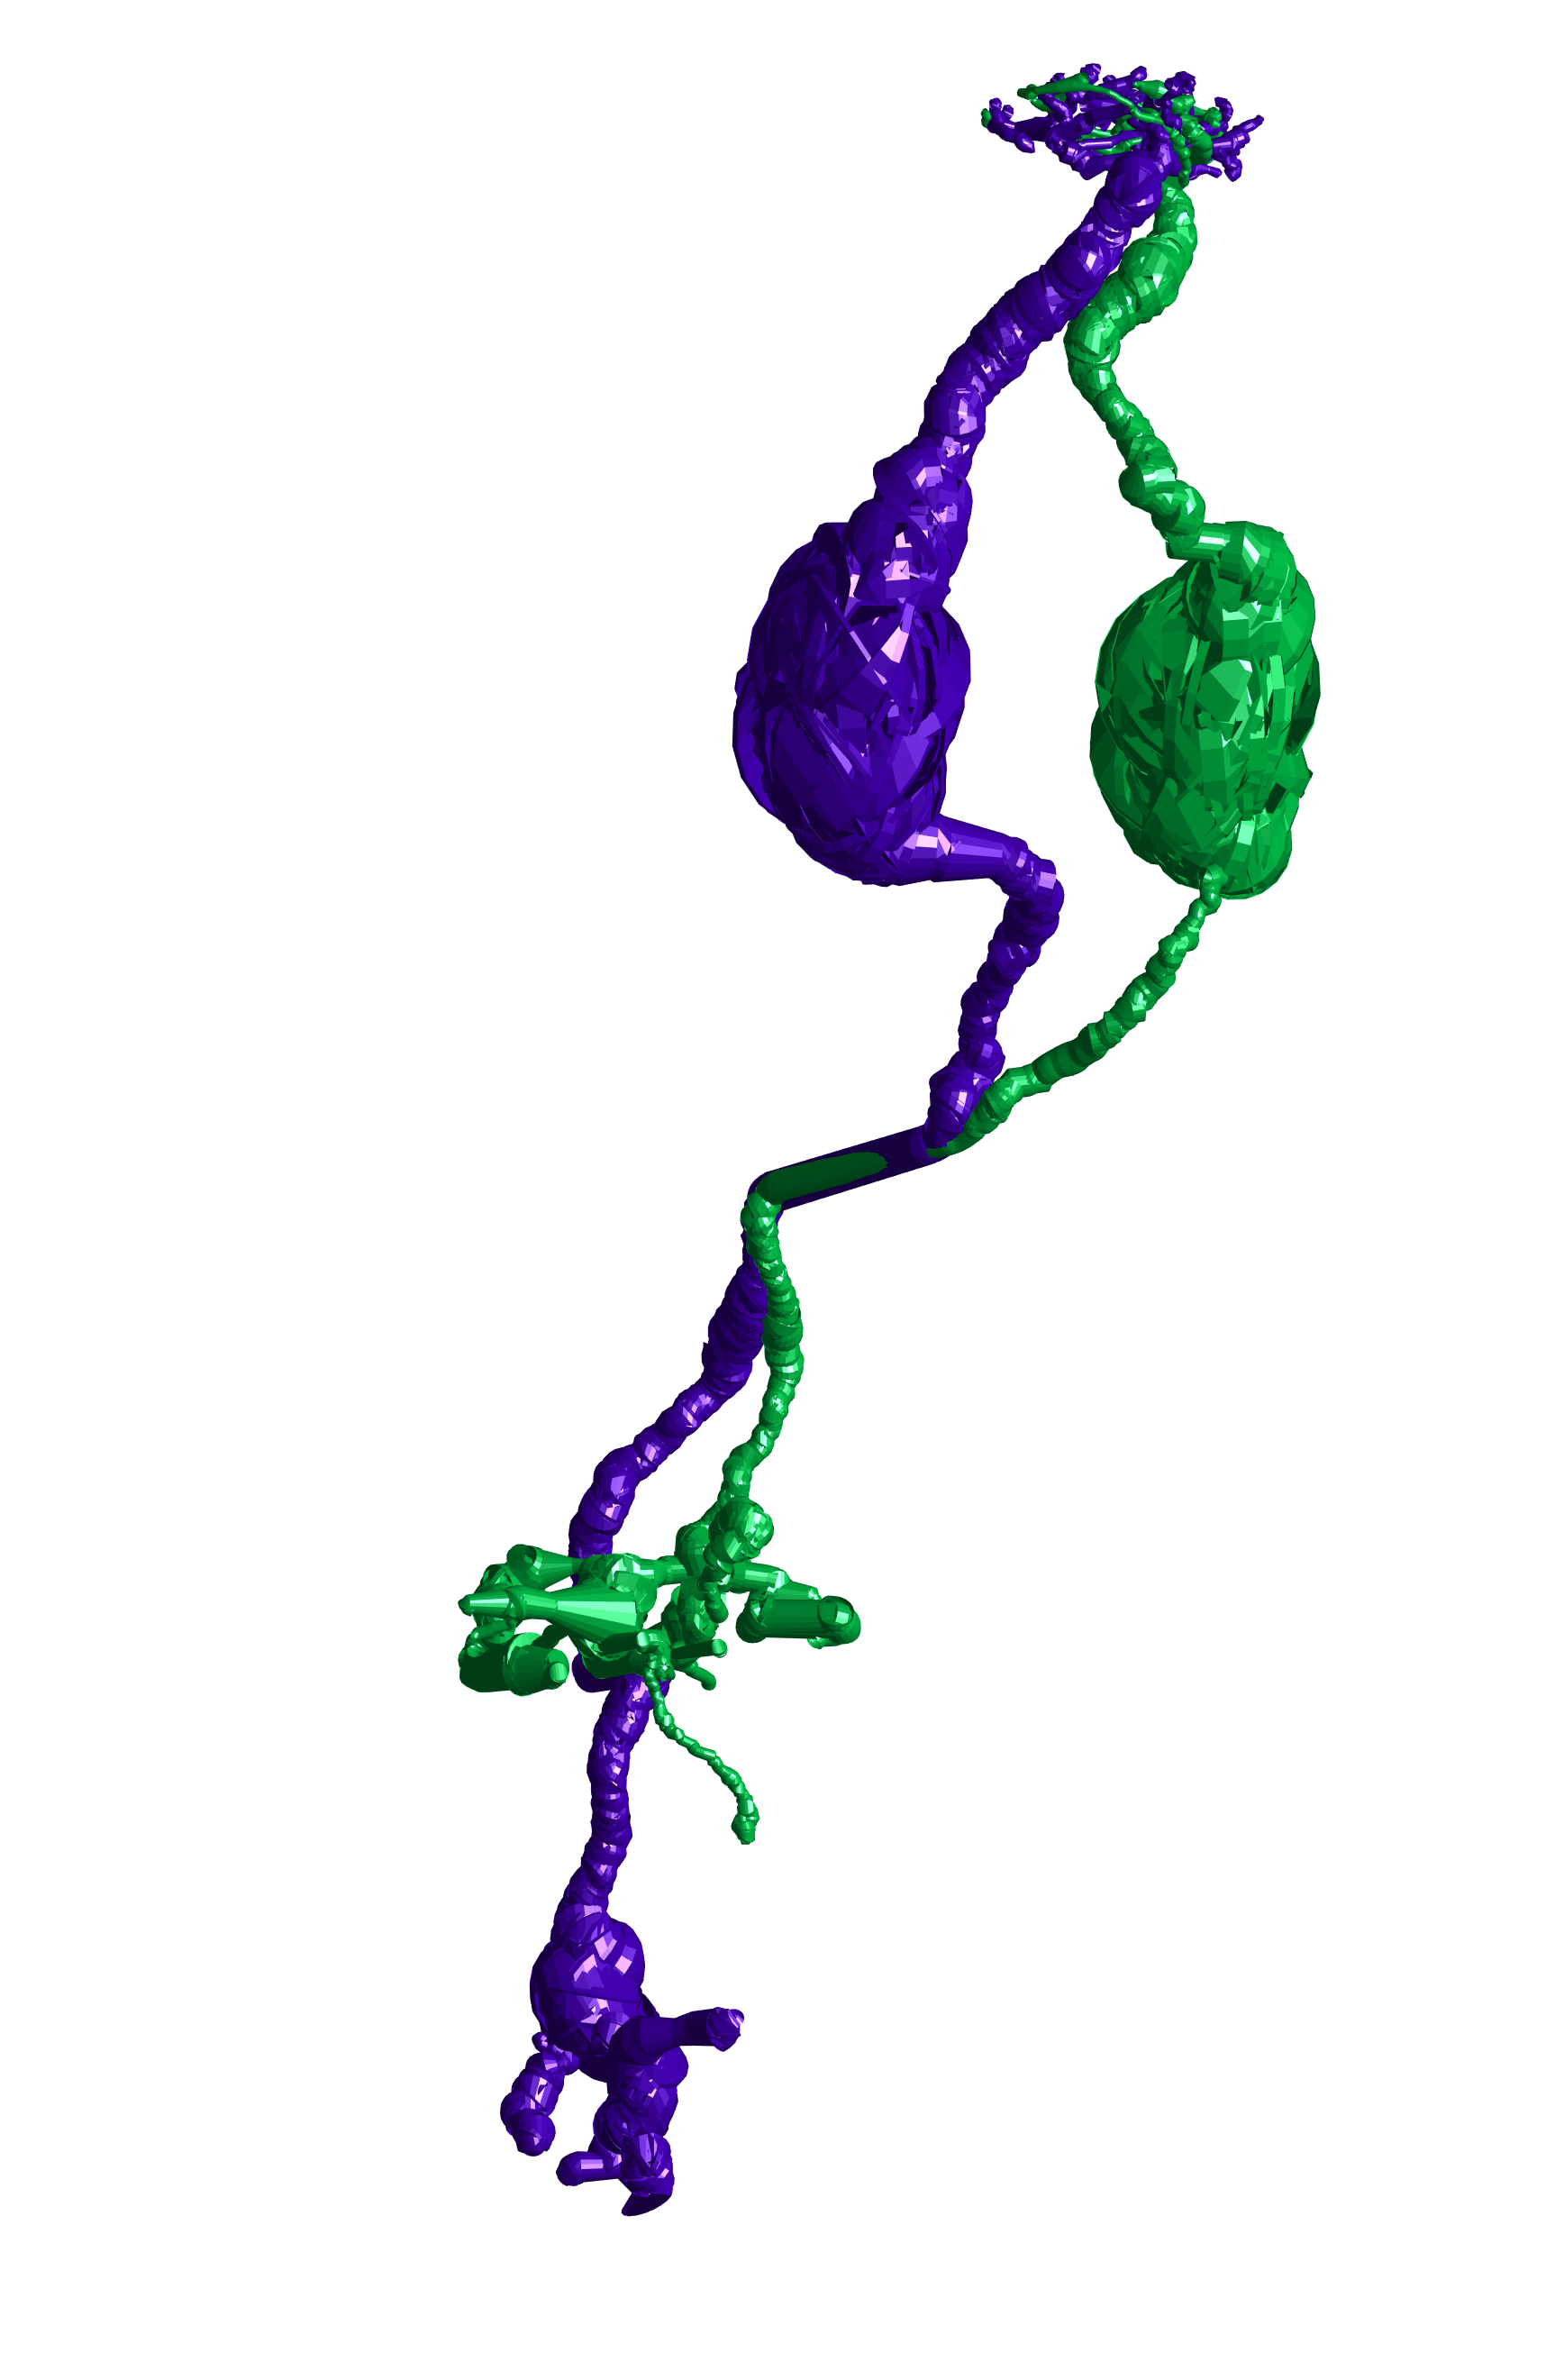
\includegraphics[width=0.5\textwidth]{midgets3D}
	\end{columns}
\end{frame}
% --------------------------------------------------- Slide --
\begin{frame}
	\frametitle{VikingPlot Comparison}
	\begin{center}
		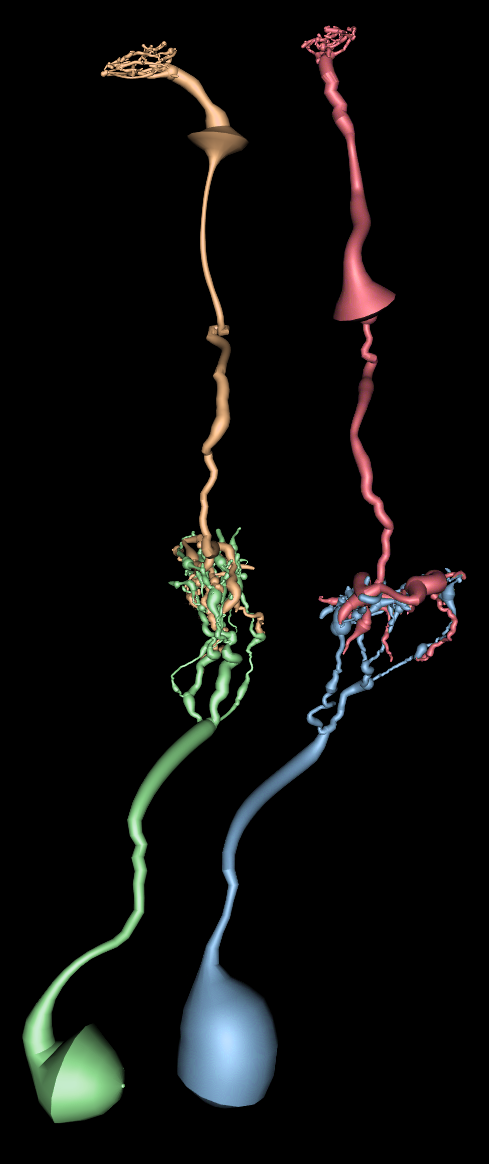
\includegraphics[height=0.7\textheight]{midgetBCGC}
		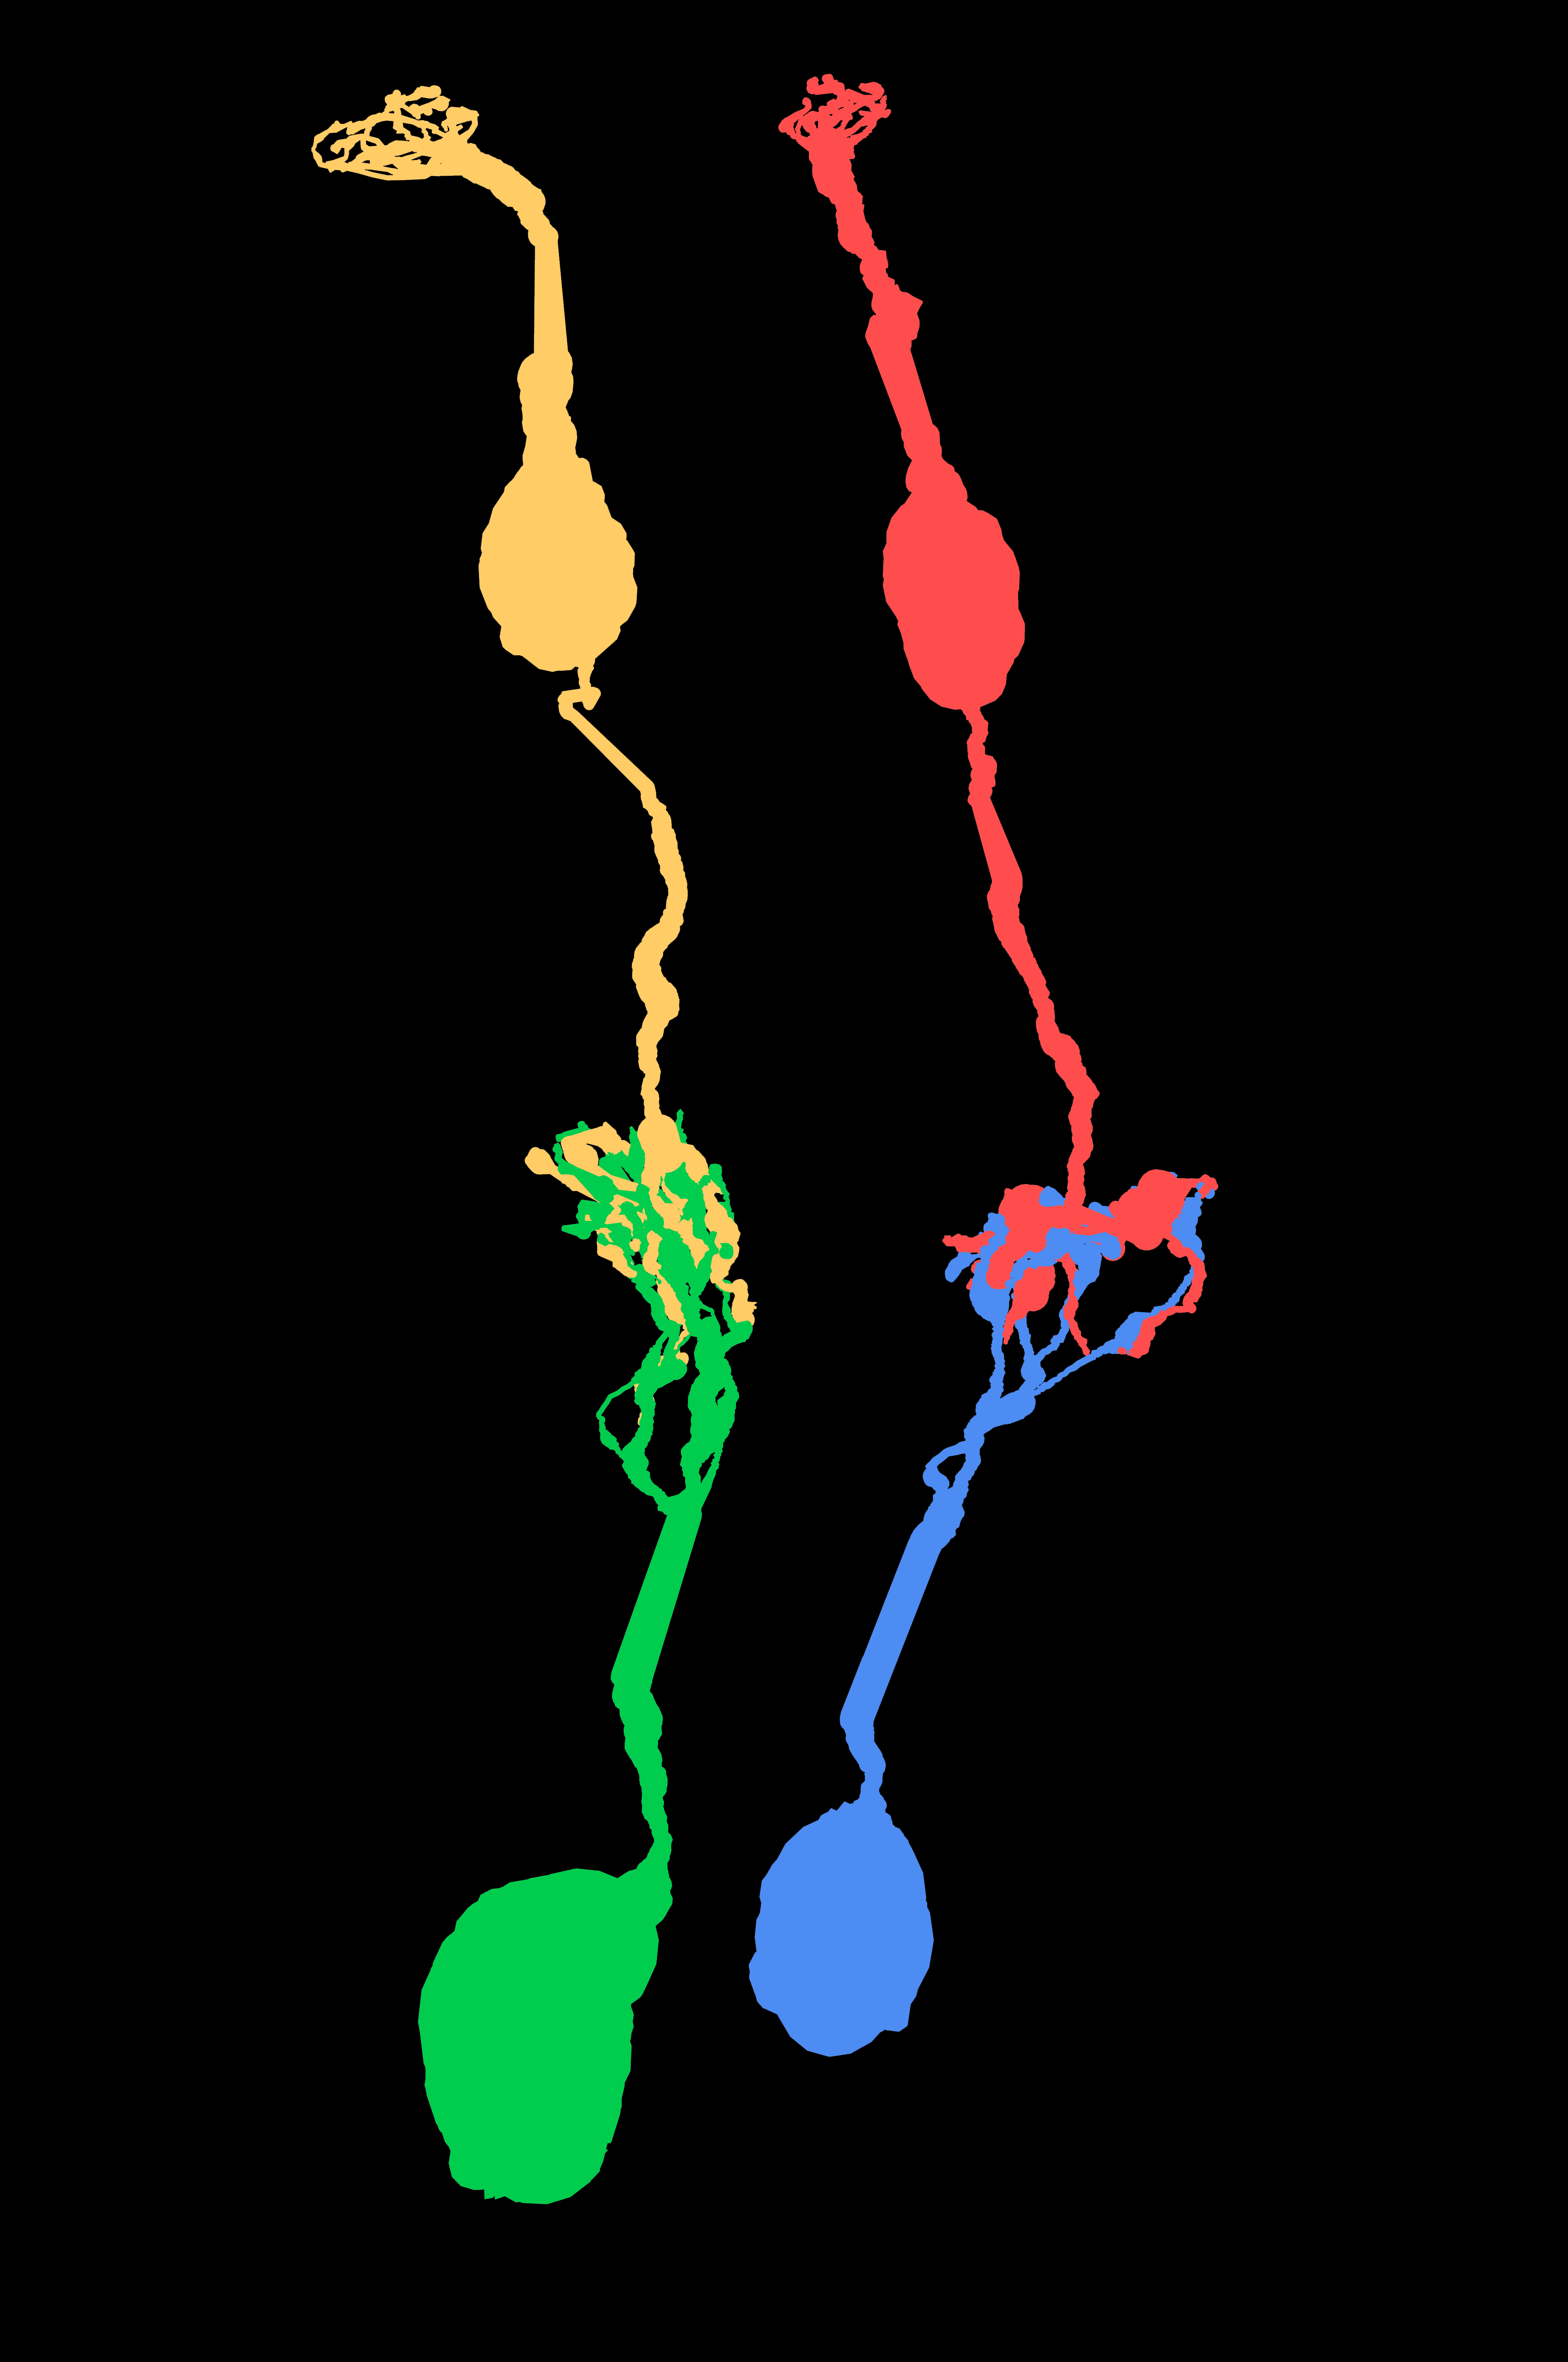
\includegraphics[height=0.7\textheight]{midgetBCGC2_k}
	\end{center}
	Efficient: This render took 32.77 sec on my laptop.
\end{frame}
% --------------------------------------------------- Slide --
\begin{frame}[fragile]
	\frametitle{Disc Renders}
	\framesubtitle{Stacked Cylinders method}
	\begin{columns}
		\column[]{0.75\textwidth}
			The Disc Render uses a similar method to the Closed Curve renders. While the result does have 3D lighting, it needs further improvement before being a viable alternative to VikingPlot or rotated cylinders.
\begin{lstlisting}[language=matlab]
c1893 = sbfsem.Neuron(1893, `i');
rodBC = sbfsem.render.Disc(1893);\end{lstlisting}
		\column[]{0.25\textwidth}
			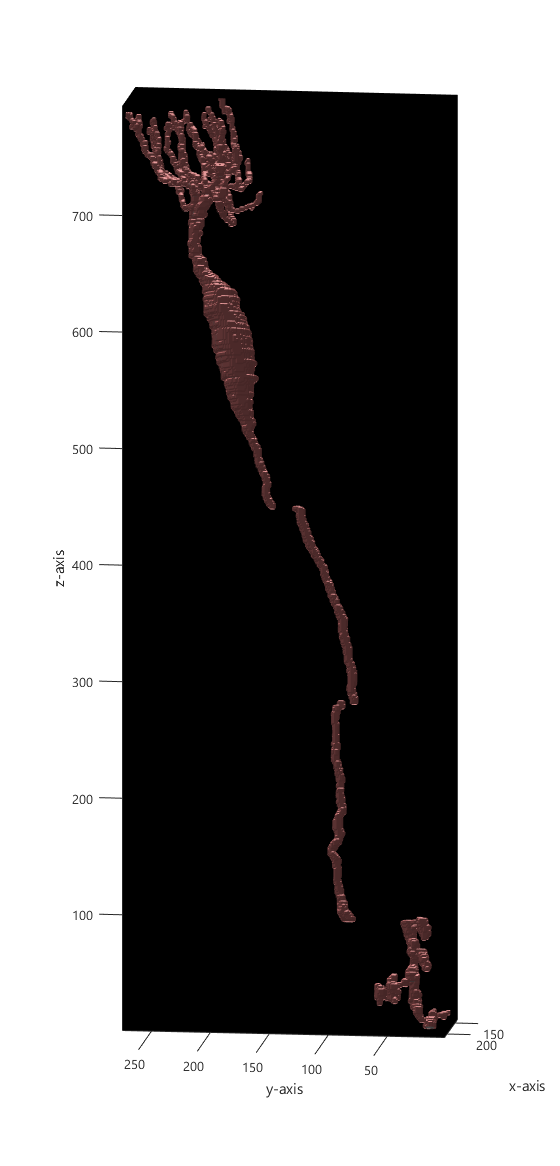
\includegraphics[width=\textwidth]{rbc}
	\end{columns}
\end{frame}
% --------------------------------------------------- Slide --
% ------------------------------------------------- Section --
\section{Export}
% --------------------------------------------------- Slide --
%\begin{frame}
%	\frametitle{Export 3D Figure to XHTML}
%	\begin{lstlisting}[language=matlab]
%	figure2xhtml('filename.xhtml');
%	% Render without lighting
%	figure2xhtml('filename.xhtml', struct('headlight', false));
%	% Add a title (Default Matlab X3 DOM)
%	figure2html('filename.xhtml', struct('title', `Your title'));\end{lstlisting}
%	The files will appear in your working directory (change with \texttt{cd()}). Click on the .xhtml file and open in your internet browser. 
%\end{frame}
% --------------------------------------------------- Slide --
% ------------------------------------------------- Section --
% ------------------------------------------------- Section --
\section{Appendix}
% ------------------------------------------------- Section --
% --------------------------------------------------- Slide --
\begin{frame}
	\frametitle{Appendix}
	Here's some information and methods that are less essential:
	\begin{enumerate}
		\item Resources
		\item Links
		\item Tulip import method
		\item Old version of NeuronApp
	\end{enumerate}
\end{frame}
% --------------------------------------------------- Slide --
% ---------------------------------------------- Subsection --
\subsection*{Links}
% ---------------------------------------------- Subsection --
% --------------------------------------------------- Slide --
\begin{frame}
	\frametitle{Links}
	The SBFSEM-tools \href{www.github.com/sarastokes/sbfsem-tools}{\textcolor{blue}{repository}} can be found on Github.\\
	The software used for annotations is \href{https://connectomes.utah.edu/}{\textcolor{blue}{Viking}}, developed by Jamie Anderson and the Marc Lab at University of Utah.\\
	Useful free programs involved in these analyses:
	\begin{itemize}
		\item \href{http://chip.de/downloads/Tulip-64-Bit_41528289.html}{\textcolor{blue}{Tulip}} supports graph visualization. The documentation for Tulip's Python package can be found \href{http://tulip.labri.fr/Documentation/4_10_0/tulip-python/html/index.html}{\textcolor{blue}{here}}.
		\item \href{http://www.blender.com}{\textcolor{blue}{Blender}} for 3D renders of neurons.
	\end{itemize}
	SBFSEM-tools was developed in the \href{http://www.neitzvision.com/}{\textcolor{blue}{Neitz lab}} at University of Washington.
\end{frame}	
% --------------------------------------------------- Slide --
% ---------------------------------------------- Subsection --
\subsection*{References}
% ---------------------------------------------- Subsection --
% --------------------------------------------------- Slide --
\begin{frame}
	\frametitle{Resources}
	3D rendering
	\begin{itemize}
		\item Lorenson \& Cline (1987) \textit{Computer Graphics}, 21(4)
		\item 3D Math Primer For Graphics and Game Development by Fletcher Dunn and Ian Parberry
		\item \href{https://www.giudansky.com/images/articoli/2016/11/xblender-infographic-1280-SM.png.pagespeed.ic.1kzexBoDEx.png}{Blender Cheatsheet}
	\end{itemize}
	OData
	\begin{itemize}
		\item \href{https://msdn.microsoft.com/en-us/library/gg334279(v=crm.7).aspx}{Microsoft Developer OData tutorials}
	\end{itemize}
	Data Structures
	\begin{itemize}
		\item \href{https://medium.com/basecs}{BaseCS}
		\item \href{https://www.cs.usfca.edu/~galles/visualization/Algorithms.html}{Data structure visualization}
	\end{itemize}
\end{frame}
% --------------------------------------------------- Slide --
% ---------------------------------------------- Subsection --
\subsection*{Tulip Import}
% ---------------------------------------------- Subsection --
% --------------------------------------------------- Slide --
\begin{frame}[fragile]
	\frametitle{Import}
	\framesubtitle{Step One: Tulip}
	\begin{block}{}
		Open a cell in Tulip and then open the Python command line. It's on the bottom toolbar.\\
		Set the file name* and file path:
		\begin{lstlisting}[language=python]
		outputFile = "C:\...\c207.json"\end{lstlisting}
		Then run these two lines:
		\begin{lstlisting}[language=python]
		params = tlp.getDefaultPluginParameters('JSON Export', graph)
		success = tlp.exportGraph('JSON Export', graph, outputFile, params)\end{lstlisting}
	\end{block}
\end{frame}
% --------------------------------------------------- Slide --
\begin{frame}
	\frametitle{Import}
	\framesubtitle{Step One: Tulip}
	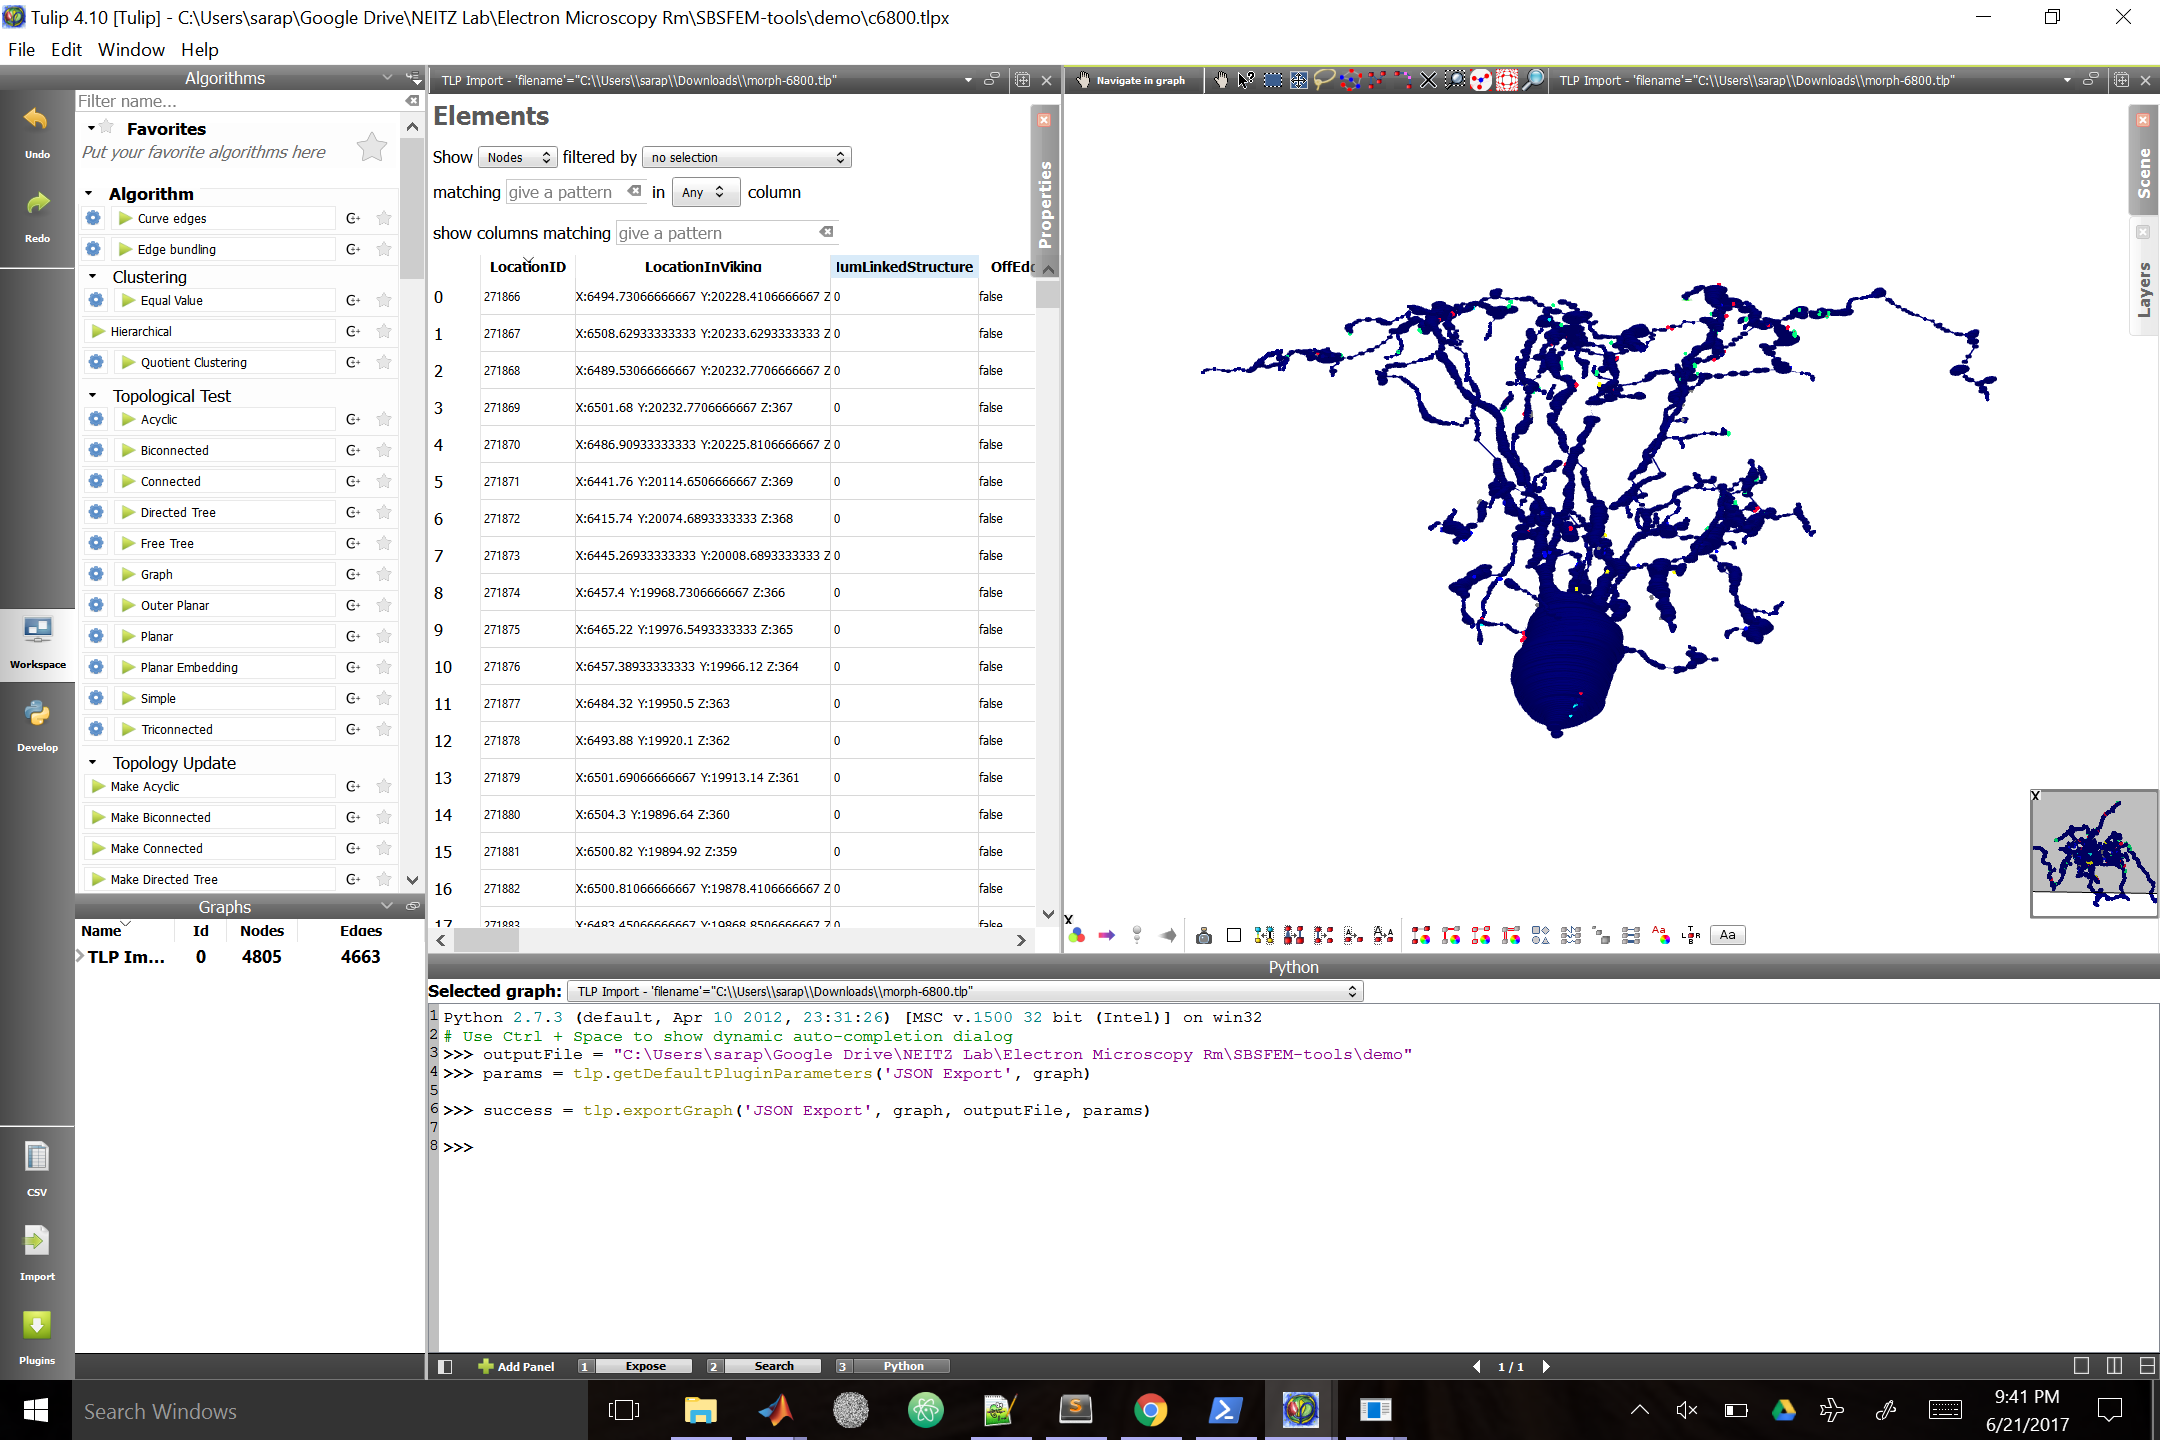
\includegraphics[width = 0.9\textwidth]{tulip_python}
\end{frame}
% --------------------------------------------------- Slide --
\begin{frame}[fragile]
	\frametitle{Alternative Streamlined Import}
	\framesubtitle{Step One - Tulip}
	If you're comfortable with Python, you can skip opening Tulip's UI entirely.\\
	First get the Tulip modules:
	\begin{lstlisting}
	$ pip install tulip-python\end{lstlisting}
	This will allow you to export \texttt{.tlp} (or compressed \texttt{.tlp.gz}) files to JSON from a command line without Tulip's UI.
	\begin{lstlisting}[language=python]
	from tulip import tlp
	graph = tlp.loadGraph("C:\...\morph-207.tlp")
	outputFile = "C:\...\c207.json"
	params = tlp.getDefaultPluginParameters('JSON Export', graph)
	success = tlp.exportGraph('JSON Export', graph, outputFile, params)\end{lstlisting}
\end{frame}
% --------------------------------------------------- Slide --
\begin{frame}[fragile]
	\frametitle{Import}
	\framesubtitle{Step Two - MATLAB}
	Load in the JSON file and create a Neuron object:
	\begin{lstlisting}[language=matlab]
	c207 = Neuron('c207.json');\end{lstlisting}
	A dialog box will ask for the cell number and source (temporal, inferior, rc1). To avoid that, include them while creating the Neuron object:
	\begin{lstlisting}[language=matlab]
	% output = Neuron(filename, cellNumber, source);
	c207 = Neuron('c207.json', 207, 'temporal');\end{lstlisting}
	To update the underlying data for an existing Neuron:
	\begin{lstlisting}[language=matlab]
	c207.updateData('c207.json');\end{lstlisting}
	Open up the user interface:
	\begin{lstlisting}[language=matlab]
	c207.openUI;\end{lstlisting}
\end{frame}
% --------------------------------------------------- Slide --
% ---------------------------------------------- Subsection --
\subsection*{NeuronApp}
% ---------------------------------------------- Subsection --
% --------------------------------------------------- Slide --
	\begin{frame}
		\frametitle{Cell Info Panel}
		This entire panel is designed with a future directory class in mind. As of now, you don't need to save each Neuron, so only set these if you have a specific reason for doing so.
		\begin{itemize}
			\item If known, the cell type and subtype will be helpful for connectivity analysis.
			\item The other properties will eventually be used for cell queries but don't have much use yet.
		\end{itemize}
			After changing any of the attributes on the Cell Info Panel, make sure to press the \texttt{[Add to cell data]} button. This will make sure your changes are reflected next time you open the UI.\\
	\end{frame}
% --------------------------------------------------- Slide --	
\begin{frame}
	\frametitle{3d plot}
	\framesubtitle{Components}
		You can add and remove each synapse type, the soma node and the skeleton independently using the checkboxes.\\Rotate the plot with the elevation and azimuth sliders.
		\vskip20pt
		\begin{columns}
			\column[]{0.5\textwidth}
				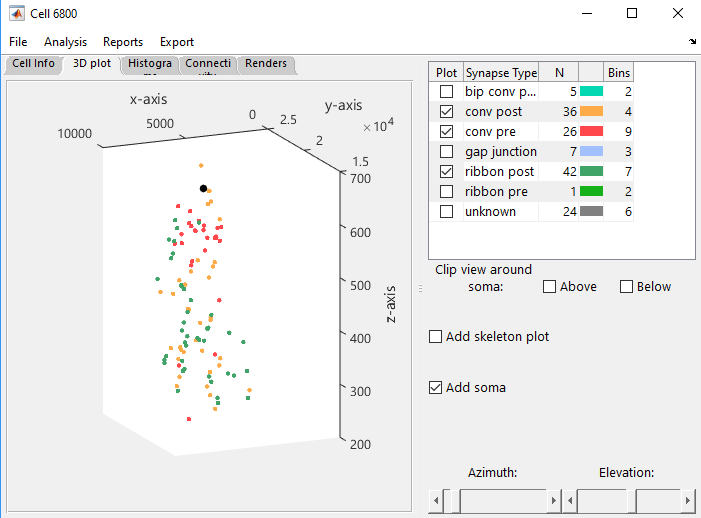
\includegraphics[width=\textwidth]{c6800_plot3}
				\vskip5pt
				AII amacrine cell synapses
			\column[]{0.5\textwidth}
				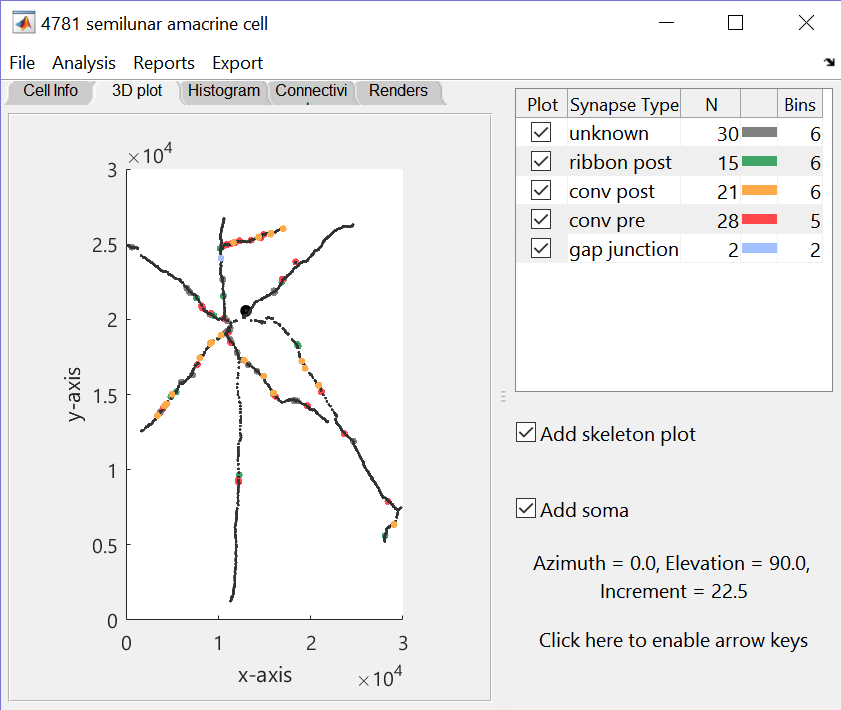
\includegraphics[width=\textwidth]{c4781_plot3}
				\vskip5pt
				Semilunar synapses \& skeleton
		\end{columns}
\end{frame}
% --------------------------------------------------- Slide --	
\begin{frame}
	\frametitle{Histograms}
	\begin{columns}
		\column[]{0.5\textwidth}
			There are two histograms. These plot synapse count as a function of:
			\begin{itemize}
				\item Distance from soma
				\item Section number (z-axis)
			\end{itemize}
		Use the Synapse Table to edit the number of bins. Add the cell skeleton to see dendrite stratification.
		\column[]{0.5\textwidth}
			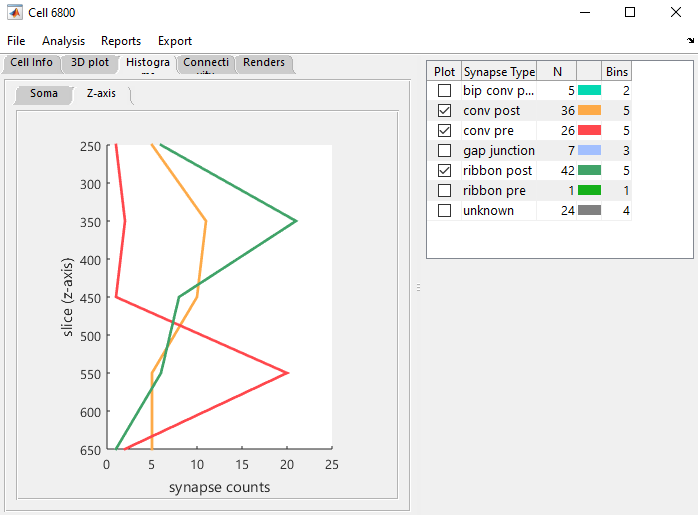
\includegraphics[width=\textwidth]{c6800_histZ}
		\vskip3pt
		Z-axis synapse distribution for a putative AII AC. This synapse asymmetry isn't news but is still good to see.
	\end{columns}
\end{frame}
% --------------------------------------------------- Slide --
\begin{frame}[fragile]
	\frametitle{Connectivity}
	To add connectivity data, save a network map in Tulip as a JSON file, as described above. Then in Matlab:
	\begin{lstlisting}[language=matlab]
c207.addConnectivity('c207hops.json');\end{lstlisting}
	\vskip10pt
	\begin{columns}
		\column[]{0.5\textwidth}
		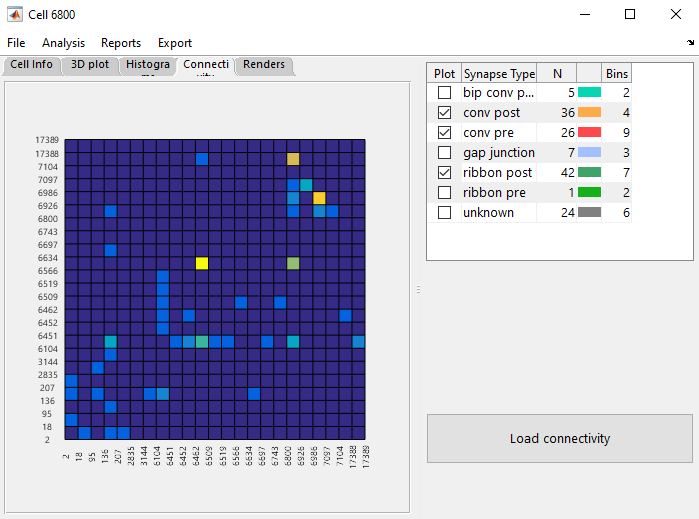
\includegraphics[height=0.4\textheight]{c6800_network}	
		\vskip10pt
		Connectivity for the AII AC.
		\column[]{0.5\textwidth}
		The connectivity matrix is weighted by the number of unique synapses between two cells (dark blue for 0 synapses). Directed synapses will only register a contact from the pre $\rightarrow$ post-synaptic neuron.
	\end{columns}
\end{frame}
% --------------------------------------------------- Slide --
\begin{frame}[fragile]
	\frametitle{Connectivity}
	The network data is split into edges and nodes, each with their own table. The tables can be exported to Excel as \texttt{.csv} or as a text file from the UI menu bar.\\
	\vskip10pt
	To print a easily readable table to the command line use the networkTable function
\begin{lstlisting}[language=matlab]
networkTable(c207);\end{lstlisting}
\end{frame}
% --------------------------------------------------- Slide --
\begin{frame}
	\frametitle{Blender Renders and Cell Fills}
	\begin{columns}
		\column[]{0.5\textwidth}
		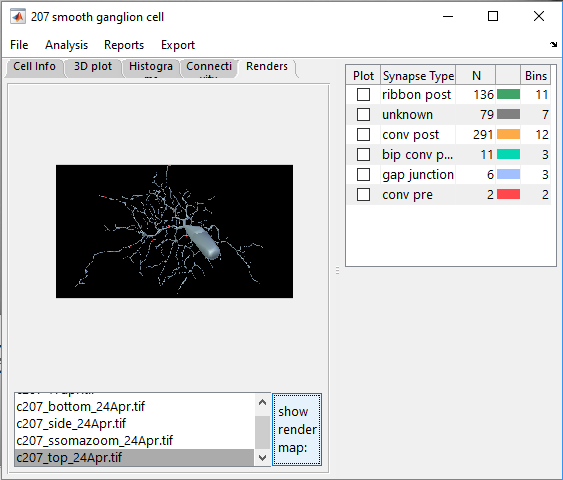
\includegraphics[width=0.9\textwidth]{c207_render}
		\hskip10pt
		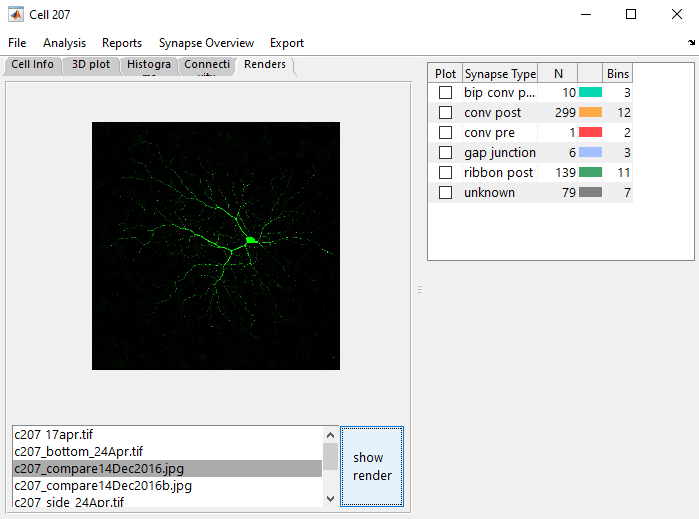
\includegraphics[width=0.9\textwidth]{c207_cellfill}
		\column[]{0.5\textwidth}
		For now, set the \texttt{renderDir} in \texttt{getFilepaths.m} to the file your images are saved into. The UI find the images if their filename includes the letter `c' followed by cell number (like `c207'). I hope to improve this at some point.
		\vskip15pt
		This isn't limited to renders and could include whatever images and diagrams are helpful. For example, I can compare my ON-smooth cell reconstructions and cell fills.
	\end{columns}
\end{frame}
% --------------------------------------------------- Slide --
\end{document}